\documentclass{article}

\usepackage{graphicx}
\usepackage{tikz}
\usepackage{tikzsymbols}
\usetikzlibrary{calc,patterns,shapes.geometric}
\pagestyle{empty}
\usepackage[margin=0pt]{geometry}
\geometry{papersize={14in,12in}}

\def\centerarc[#1](#2)(#3:#4:#5){\draw[#1] ($(#2)+({#5*cos(#3)},{#5*sin(#3)})$) arc (#3:#4:#5);}

\begin{document}
	\begin{figure}
		\centering
		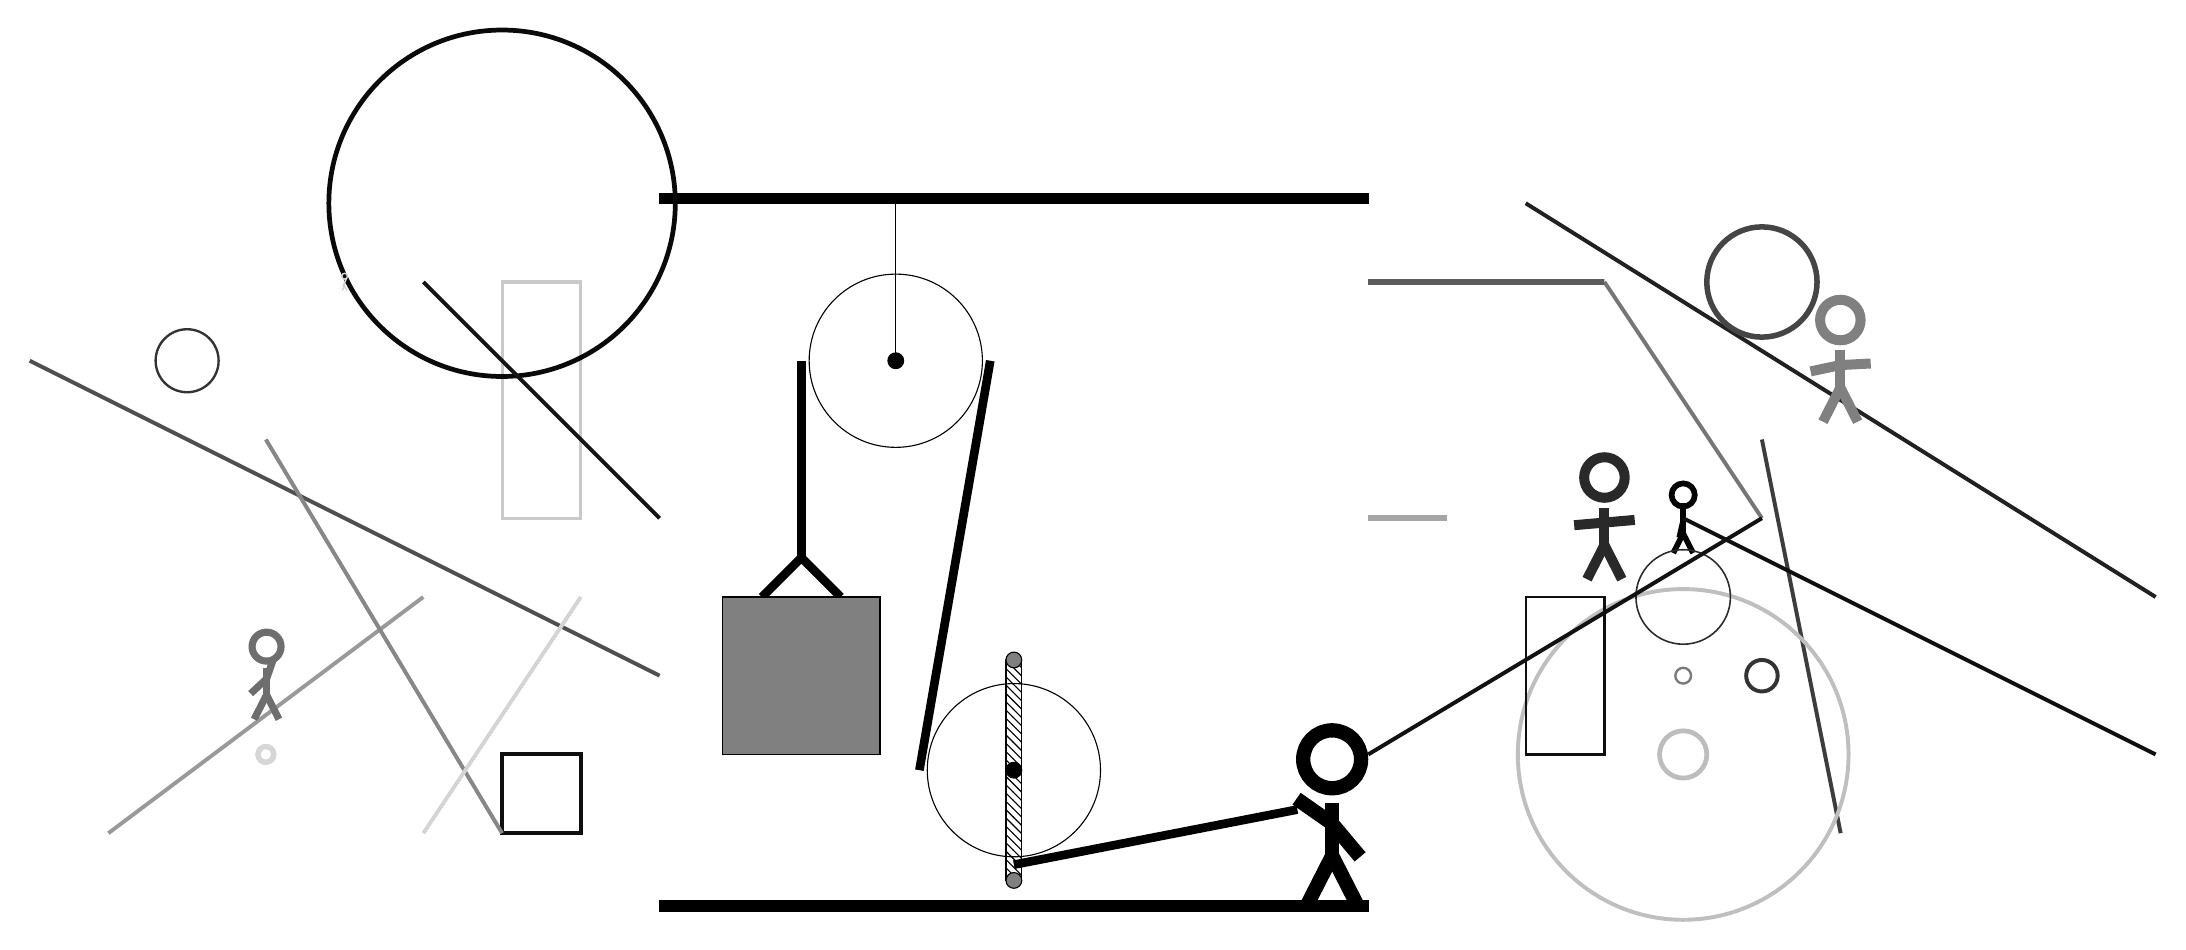
\begin{tikzpicture}
			%%%%% START %%%%%
			
			\draw[fill=black] (-2, 9) rectangle (7, 9.125);
			
			\draw (1, 7) circle (1.1);
			\draw[fill=black] (1, 7) circle (0.1);
			\draw (1, 9) -- (1, 7);
			
			\draw[fill=white](2.5, 1.8) circle (1.1);
			\draw[fill=black] (2.5, 1.8) circle (0.1);
			\draw[pattern=north west lines, pattern color=black] (2.4, 3.2) rectangle (2.6, 0.4);
			\draw[fill=black!50] (2.5, 3.2) circle (0.1);
			\draw[fill=black!50] (2.5, 0.4) circle (0.1);
			
			\draw[line width=1.1mm] (-0.7, 4.0) -- (-0.2, 4.5) -- (0.3, 4.0);
			\draw[fill=black!50] (-1.2, 4.0) rectangle (0.8, 2.0);
			
			\draw[line width=1.1mm] (-0.2, 7) -- (-0.2, 4.5);
			\centerarc[line width=1.1mm](1, 7)(0:180:1.2000000000000002);
			\draw[line width=1.1mm](2.2, 7) -- (1.3, 1.8);
			\centerarc[line width=1.1mm](2.5, 1.8)(180:270:1.2000000000000002);
			\draw[line width=1.1mm](2.5, 0.6) -- (6.1, 1.3);
			
			\draw[line width=0.4mm, color=black!21] (-3, 8) rectangle (-4, 5);
			
			\draw [line width=0.6mm, color=black!96](-4, 9) circle (2.2);
			\node[line width=0.7mm, color=black!99] at (11, 5) {\Strichmaxerl[4][77][90]};
			\draw[line width=0.5mm, color=black!54](12, 5) -- (10, 8);
			\draw[line width=0.5mm, color=black!12] (-3, 1) rectangle (-3, 1);
			
			\draw[line width=0.5mm, color=black!40](-5, 4) -- (-9, 1);
			\draw[line width=0.5mm, color=black!76](12, 6) -- (13, 1);
			\draw [line width=0.3mm, color=black!80](-8, 7) circle (0.4);
			\draw[line width=0.5mm, color=black!87](9, 9) -- (17, 4);
			\draw[line width=0.5mm, color=black!69](-2, 3) -- (-10, 7);
			
			\node[line width=0.3mm, color=black!57] at (-7, 3) {\Strichmaxerl[5][43][71]};
			
			\draw[line width=0.5mm, color=black!94](11, 5) -- (17, 2);
			\draw [line width=0.5mm, color=black!80](12, 3) circle (0.2);
			
			\draw [line width=0.5mm, color=black!25](11, 2) circle (2.1);
			\draw [line width=0.7mm, color=black!16](-7, 2) circle (0.1);
			\draw [line width=0.2mm, color=black!83](11, 4) circle (0.6);
			\draw[line width=0.5mm, color=black!94] (-4, 2) rectangle (-3, 1);
			
			\node[line width=0.4mm, color=black!17] at (-6, 8) {\Strichmaxerl[1][64][65]};
			\draw[line width=0.7mm, color=black!35] (8, 5) rectangle (7, 5);
			\draw [line width=0.6mm, color=black!26](11, 2) circle (0.3);
			\node[line width=0.3mm, color=black!50] at (13, 7) {\Strichmaxerl[7][12][3]};
			
			\draw [line width=0.3mm, color=black!52](11, 3) circle (0.1);
			\draw[line width=0.5mm, color=black!92](-5, 8) -- (-2, 5);
			\draw[line width=0.5mm, color=black!93](7, 2) -- (12, 5);
			\draw[line width=0.3mm, color=black!94] (9, 4) rectangle (10, 2);
			\node[line width=0.6mm, color=black!84] at (10, 5) {\Strichmaxerl[7][5][5]};
			
			\draw[line width=0.5mm, color=black!45](9, 6) -- (9, 6);
			\draw[line width=0.5mm, color=black!47](-4, 1) -- (-7, 6);
			\draw [line width=0.7mm, color=black!73](12, 8) circle (0.7);
			
			\draw[line width=0.5mm, color=black!17](-5, 1) -- (-3, 4);
			\draw[line width=0.7mm, color=black!64] (7, 8) rectangle (10, 8);
			
			\node at (6.5, 1.2) {\Strichmaxerl[10][-35][-50]};
			
			\draw[fill=black] (-2, 0) rectangle (7, 0.15);
			
			%%%%% END %%%%%
		\end{tikzpicture}
	\end{figure}	
\end{document}